\documentclass{anstrans}
%%%%%%%%%%%%%%%%%%%%%%%%%%%%%%%%%%%
\title{Parallel Performance and Application of the Time Dependent Transport Code TDKENO }
\author{Zander Mausolff,$^{*}$ Mark DeHart,$^{\dagger}$ Sedat Goluoglu $^{*}$}

\institute{
$^{*}$Nuclear Engineering Program, University of Florida
\\
529 Gale Lemerand Dr., Gainesville, FL, 32611
\and
$^{\dagger}$Nuclear Systems Design and Analysis Department Idaho National Laboratory 
\\
2525 North Freemont Street, Idaho Falls ID, 83415
}

\email{zanderm@ufl.edu $^{*}$} 


% Optional disclaimer: remove this command to hide
%\disclaimer{Notice: this manuscript is a work of fiction. Any resemblance to
%actual articles, living or dead, is purely coincidental.}

%%%% packages and definitions (optional)
\usepackage{graphicx} % allows inclusion of graphics
\usepackage{booktabs} % nice rules (thick lines) for tables
\usepackage{microtype} % improves typography for PDF

\newcommand{\SN}{S$_N$}
\renewcommand{\vec}[1]{\bm{#1}} %vector is bold italic
\newcommand{\vd}{\bm{\cdot}} % slightly bold vector dot
\newcommand{\grad}{\vec{\nabla}} % gradient
\newcommand{\ud}{\mathop{}\!\mathrm{d}} % upright derivative symbol

\begin{document}
%%%%%%%%%%%%%%%%%%%%%%%%%%%%%%%%%%%%%%%%%%%%%%%%%%%%%%%%%%%%%%%%%%%%%%%%%%%%%%%%
\section{Introduction}
Renewed interest in high fidelity simulation of excursion events has prompted the improvement of many codes that solve the time dependent transport equation. Often these codes make approximations to the transport equation in order to achieve results in a reasonable amount of time.  One method, the improved quasi-static (IQS) method is the most accurate compared to adiabatic, diffustion, point kinetics, etc., but requires several expensive calculations for the flux shape.  The code TDKENO employs the IQS method. To minimize the computational time associated with the flux shape calculation, a modified version of KENO from Scale 6.2 is employed. This version of KENO runs in parallel across hundreds of nodes enabling drastically lower computational time.

The parallel capabilities of KENO allow TDKENO to simulate complex transient experiments with a large number of histories. The primary application of these improvements is the simulation of TREAT calibration experiments to aid in the restart and provide reference calculation for other codes. We present the improved computational overhead, memory usage, and accuracy for TDKENO in the case of simulating the entire TREAT core. 

%%%%%%%%%%%%%%%%%%%%%%%%%%%%%%%%%%%%%%%%%%%%%%%%%%%%%%%%%%%%%%%%%%%%%%%%%%%%%%%%
\section{Theory}
Solving the transport equation is non trivial when including the time dependence and explicit representation of delayed neutrons.  Utilizing the IQS method relies on the assumption that the total neutron flux is factored into a shape and amplitude function.  The amplitude function is highly time dependent solves the point kinetics equations using the  the inner product definitions of reactivity, generation time, etc.  Whereas the shape function varies slowly in time and solves a modified version of the steady state transport equation.  In TDKENO the shape equation is solved via Monte Carlo, but in general the shape equation may be solved other ways.  This factorization and corresponding normalization can be found in refs. (Henry,Bently,Otto,etc.).  

Applying this factorization to the three dimensional time dependent transport equation with the explicit representation of delayed neutrons results in a set of coupled equations. A complete derivation is readily found in [Bentley, etc].  Equations for the flux shape, amplitude, and delayed neutron precursors are solved on several time scales through an iterative process. 

\begin{figure}[h]
    \centering
    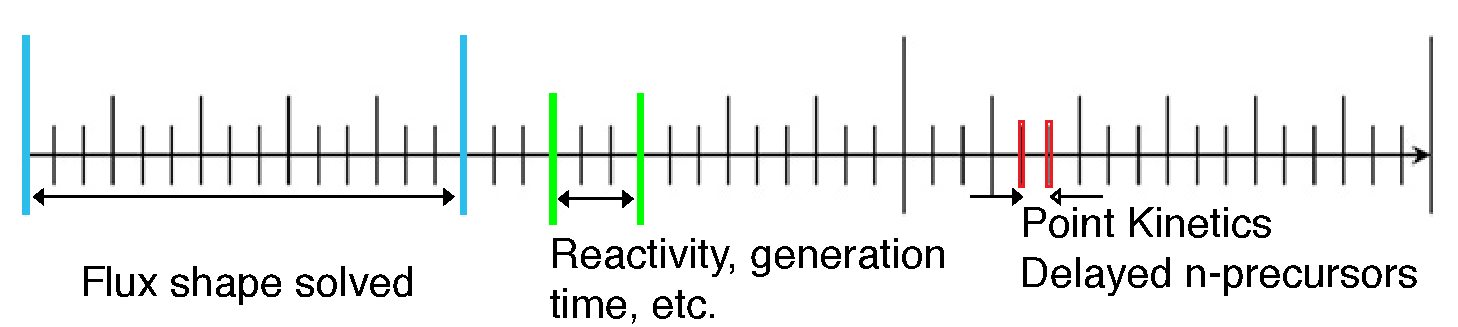
\includegraphics[width=8cm]{figures/time_scale.pdf}
    \caption{Time scale variation for IQS.}
    \label{fig:time_scale}
\end{figure}

The advantage of these varying time scales is computational savings.  This comes from the flux shape being solved on a large time steps and only done when the spatial distribution of neutrons changes significantly.  In between flux shapes the corresponding differential equations are solved to capture the time dependent behaviour.  Reactivity, generation time, and delayed neutron fraction are found from their inner product definitions and fed into the point kinetics equations.  Alternatively these values may be computed during the Monte Carlo random walk but required significant neutron histories to achieve low uncertainties (Waddell). In some IQS implementations there are tests to determine if the time step is too large to solve the flux shape over (Dulla). 

\begin{figure}[h]
    \centering
    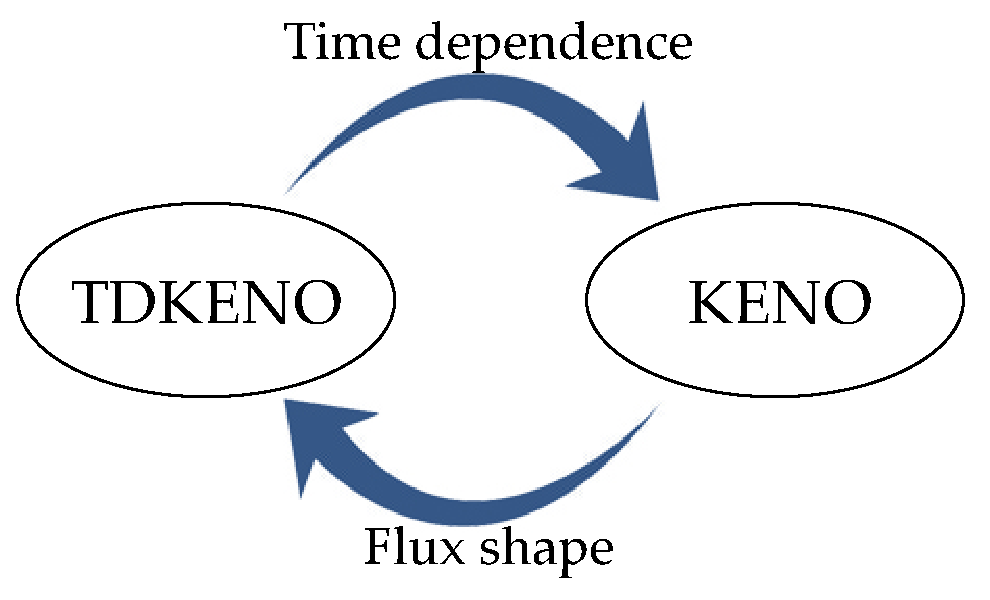
\includegraphics[width=7cm]{figures/tdkeno_flow.pdf}
    \caption{Relationship between TDKENO and KENO.  TDKENO drives the time dependence, getting the spatial neutron distribution from KENO.}
    \label{fig:tdkeno_flow}
\end{figure}

 In its current formulation, TDKENO does not do this but rather lets the user define when the a flux shape should be calculated.  This gives flexibility and may allow for computational savings as transients often experience a rapid change in neutron distribution and rapidly come to a steady state therefore not requiring a new calculation of the flux shape. However, since taking too large of a step is a possibility and may result in less quality answer, we are motivated to study the affects of varying the number of shape calculations prescribed.

%Equations look exceedingly pretty. Here is a 3-D, monoenergetic, steady-state
%transport equation with isotropic scattering and an isotropic extraneous source:
%\begin{subequations} \label{eqs:fullTransport}
%\begin{multline} \label{eq:fullTransportVol}
%  \vec{\Omega}\vd \grad \psi(\vec{x}, \vec{\Omega})
%  + \sigma(\vec{x}) \psi (\vec{x}, \vec{\Omega})
%\\ =
%  \frac{\sigma_s(\vec{x})}{4\pi} \int_{4\pi} \psi(\vec{x},\vec{\Omega}')
%  \ud\Omega' + \frac{q(\vec{x})}{4\pi}
%  \equiv \frac{1}{4\pi} Q(\vec{x}) \,,
%\end{multline}
%inside $\vec{x} \in V$, $\vec{\Omega} \in 4\pi$, with an incident boundary
%condition
%\begin{equation} \label{eq:fullTransportBndy}
%  \psi(\vec{x}, \vec{\Omega}) = \psi^b(\vec{x}, \vec{\Omega}) \,,
% \quad \vec{x} \in \partial V, \ \vec{\Omega} \vd \vec{n} < 0\,.
%\end{equation}
%\end{subequations}

%%%%%%%%%%%%%%%%%%%%%%%%%%%%%%%%%%%%%%%%%%%%%%%%%%%%%%%%%%%%%%%%%%%%%%%%%%%%%%%%
\section{Results and Analysis}
With the integration of the latest version of KENO from SCALE 6.2 we now have the ability to calculate the most intensive portion of the calculation in parallel.  Previously for problems with complex geometry the calculation of the shape may have taken several days to weeks when using to achieve adequate sampling and statistics.  By running TDKENO at the University of Florida's HiperGator supercomputer we are able to run on hundreds of CPUs resulting in the same calculations taking several hours.  These improvements are illustrated by comparing the time and memory usage with parallel KENO.  We apply these improvements to a particularly challenging problem of modeling the transients experiments with the Transient Reactor Test Facility (TREAT).  Without verification the time steps taken in TDKENO are suitable for this problem we vary the frequency of flux shape and point kinetics calculations.

To evaluate the perforance of these improvements to TDKENO we run a simulation of one of the M8CAL experiments on varying numbers of nodes on UF's Hiper gator.  Each node has an Intel E5-2698 v3 (16 core, 2.3 GHz) with 4GB of ram per node.  We note, at present only the flux shape is calculated in parallel.  The point kinetics calculations are all done in serial and are being invesitaged on the possiblity of calculating these quantities on graphics cards.  The M8CAL experiment is refereed to in the documentation of the temperature limited transient #2855 (M8CAL reference).  This one was chosen as it acutally has been the most difficult to simulate compared to similar transients, referred to as #2856 and #2857. In previous modeling of these experiments the experimental data compared to was thought to have inconsistencies with the values reported in the write up (my PHYSOR 2016 paper).  However, upon further inspection the data that corresponds to the M8CAL reported values has been found, digitized and compared to the results shown here.



%%%%%%%%%%%%%%%%%%%%%%%%%%%%%%%%%%%%%%%%%%%%%%%%%%%%%%%%%%%%%%%%%%%%%%%%%%%%%%%%
\subsection{Computational Improvements}

The computaional improvements are highlighted in TDKENO by comparing the same problem run on an increasing number of cores.  In this case the KENO calculations were run with 10000 particles per generation with a total of 2500 generations. A total of 14 flux shapes were calculated with KENO at times cenetered around the first few seconds.  We have chosen these numbers as it appears to give almost identical results to simulations run with many more histories as seen in Figure \ref{compare_hist}.  Simulations run with additional histories do result in less statistical uncertainties in values such as fluxes, keff, etc.  These are of less interest in this paper.  The model of the TREAT core used contains approximately 4000 regions with 21 materials using KENO-VI generalized geometry.  The TREAT core is unique in its ability to safely have simulate large reactivity insertions.  It accomplishes this with a core composed of 93.1\% U02 within a graphite matrix, with a ratio of U02 to graphite of 1:10000.  Details about the TREAT core may be found in (TREAT refs).  A variety of control rods are available and the transient shown in this paper is induced by the rapid withdrawl of transient rods over 0.13 seconds. 

\begin{figure}
\label{compare_hist}

\caption{Figure comparing calculated values with a varying number of histories.}
\end{figure}

Below we show the affect of increasing the number of cores the problem is run on.  The relatively low number of histories results in poor scaling to large number of cores due to increased communication time and less work done by each core.  The communication time is compounded because the flus shape calculation is done in parallel with the results gathered on the master.  This master processor then computes the point kinetics values in serial and thus are not improved with the integration of parallel KENO.  Nevertheless the perofrmance is drastically improved when compared to serial with a modest amount of processors (for high performance computing standards).  
\begin{table}[h]
    \centering
    \begin{tabular}{c|c|c}
                    Total Cores & Memory & Elapsed Time (minutes) \\
                    1           &        &   12347            \\  
                    16          &        &                \\  
                    32          &        &   1619              \\  
                    48          &        &   1356              \\  
                    64          &        &   1051             \\  
                    80          &        &                \\  
                    96          &        &   917             \\  
    \end{tabular}
    \caption{Variation of the number of cores run for the simulation of #2855. Elapsed time generated from the SLURM submission system. }
    \label{tab:parallel}
\end{table}
The poor parallel efficiency is further evidenced when inspecting the efficiency as measured by KENO for a single flux shape.  


%%%%%%%%%%%%%%%%%%%%%%%%%%%%%%%%%%%%%%%%%%%%%%%%%%%%%%%%%%%%%%%%%%%%%%%%%%%%%%%%
\subsection{Flux Shape Variation}
M8CAL 2855 only?

\begin{table}[h]
    \centering
    \begin{tabular}{c|c|c}
         & TDKENO-K5 & TDKENO-K6 \\
        Generations &  10000 & 10000 \\
        Particles   &  10000 & 10000 \\
        Skipped     &  500   & 500  \\
    \end{tabular}
    \caption{Caption}
    \label{tab:my_label}
\end{table}

\subsection{Point Kinetics Variation}
As mentioned the IQS methodology empolyed splits the transport equation into several coupled equations solved on 3 time scales.  Two of these scales relate to the solving of the point kinetics equation.  The shortest involves finding the values for reactivity, generation time, etc. from each quantitties respective inner productive definition.  These definitinos are readily available and can be found in (ref Bently?).  The differential equation formed from these qauntites is solved on a larger time scale.  Both the frequency of the updates to these inner product values and the point kinetics equation may be varied. These values are easier to find than the flux shape and thus are solved considerably more frequently. These too are formulated to contain the time dependence and must be solved when the system is undergoing significant changes (e.g. reactivity insertion). 

To determine the minimum number of times to solve the point kinetics equation between flux shape updates perform several simulations.  Each simulation we increase the number of times the quantities within the point kinetics equation are evaluated until the behavior appears to not change.  The quantity of most interest in these transient experiments is the total energy deposited in the core, thus is a number we would like to simulate accurately.  Additionally, experimental values for the yield are reported for this experiment.  Both experimental and all calculated values for the yield as function of time are found in Figure \ref{fig:var_pt_kin}.  The first few calculations (ptkin10)  

\begin{figure}
\label{fig:var_pt_kin}

\caption{Varitaion of point kinetics and comparison to experiment.}

\end{figure}

%%%%%%%%%%%%%%%%%%%%%%%%%%%%%%%%%%%%%%%%%%%%%%%%%%%%%%%%%%%%%%%%%%%%%%%%%%%%%%%%
\section{Conclusions}


%%%%%%%%%%%%%%%%%%%%%%%%%%%%%%%%%%%%%%%%%%%%%%%%%%%%%%%%%%%%%%%%%%%%%%%%%%%%%%%%

%%%%%%%%%%%%%%%%%%%%%%%%%%%%%%%%%%%%%%%%%%%%%%%%%%%%%%%%%%%%%%%%%%%%%%%%%%%%%%%%
\section{Acknowledgments}
This material is based upon work supported the Idaho National Laboratory.

%%%%%%%%%%%%%%%%%%%%%%%%%%%%%%%%%%%%%%%%%%%%%%%%%%%%%%%%%%%%%%%%%%%%%%%%%%%%%%%%
\bibliographystyle{ans}
\bibliography{bibliography}



\end{document}

